% BEGIN REVISION
{\revisioncmd
\section{Memory Relations of \ccm{}}
\label{sec:overview-verification:injection}

\ccm{} uses the original memory identity and extension of \cc{}
(\Cref{sec:overview-verification:injection:original}) and mildly
strengthens the original memory injection to reason about dynamically allocated
local memory such as a function's stack frame for \emph{open} modules,
which can be compared to the structured injection of \ccc{}
(\Cref{sec:overview-verification:injection:dynamic}).
Moreover, we generalize it further to reason about statically allocated local memory
such as static variables of C by allowing module-local invariants on those static variables
(\Cref{sec:overview-verification:injection:static}).

\subsection{Enriched Memory Injection}
\label{sec:overview-verification:injection:dynamic}
%
For open modules, reasoning about dynamically allocated local memory
such as a function's stack frame requires to strengthen the original
memory injection due to the presence of unknown modules.  The reason
is because when reasoning about a module $M$, we have to assume that
an unknown function invoked by $M$ does not change the dynamic local
memory of $M$ and also guarantee that a function of $M$ invoked by an
unknown module does not change the caller's dynamic local memory.

For this purpose, \ccc{} introduces \emph{structured injections} that
enrich the original memory injections with ownership information (\ie
whether owned by the current module or others) for all memory blocks
including public ones.  Using them, structured simulations impose
fine-grained invariants subject to the ownership information and a
concrete leakage protocol based on reachability from pointers.

Unlike \ccc{}, \ccm{} generalizes open simulations and memory injections
in a more abstract way following \cite{DBLP:conf/icfp/DreyerNB10,pb}.

First, we generalize the external call case of the open simulation in \Cref{fig:open-sim}
by allowing \emph{private transitions}, denoted $\sqsupseteq_\weak$,
as follows (\textcolor{red}{in red color}):
\[
\begin{array}{@{}l@{}}
\texttt{ 5:}~\quad \textcolor{red}{\exists w' \sqsupseteq_\weak w},~ (f_\src,f_\tgt)\in \texttt{vrel}(\textcolor{red}{w'}) \land (\vec{v}_\src,\vec{v}_\tgt) \in \overrightarrow{\texttt{vrel}(\textcolor{red}{w'})} \land{} \\[1mm]
\texttt{ 6:}~\quad \textcolor{red}{\forall w'' \sqsupseteq w'},~\forall (\memsrc',\memtgt')\in\texttt{mrel}(\textcolor{red}{w''}),~ \forall (r_\src,r_\tgt)\in \texttt{vrel}(\textcolor{red}{w''}),\\[1mm]
\texttt{ 7:}~\quad \textcolor{red}{\exists w''' \sqsupseteq_\weak w'',~ w''' \sqsupseteq w} \land {} \\
\phantom{\texttt{ 7:}}~\quad ((\memsrc',\mathtt{after\_external}~r_\src~\stsrc),(\memtgt',\mathtt{after\_external}~r_\tgt~\sttgt))\in R(\textcolor{red}{w'''})
\end{array}
\]
Though private transitions are allowed before and after an external function call (\ie
$w' \sqsupseteq_\weak w$ and $w''' \sqsupseteq_\weak w''$),
the overall transition should be \emph{public} (\ie $w''' \sqsupseteq w$)
assuming the external call also makes a public transition (\ie $w'' \sqsupseteq w'$).%
\footnote{We only allow private transitions just before and after external calls for simplicity.
See \Cref{sec:related} for comparison with \cite{DBLP:conf/icfp/DreyerNB10,pb}.}

Second, we extend memory injections to specify others' dynamic local
memories in the source and target that should be unchanged by the current module.
Specifically, an (enriched) memory injection $(\iota, m^\weak_\src, m^\weak_\tgt)$
consists of an original memory injection $\iota$ mapping the source public blocks into target blocks; and additionally
a private (\ie dynamic local) memory of the source $m^\weak_\src$ and that of the target $m^\weak_\tgt$
where $m^\weak_\src$ and $m^\weak_\tgt$ should be disjoint from the public memories specified by~$\iota$.
Then, private transitions from $(\iota, m^\weak_\src, m^\weak_\tgt)$ to
$(\iota', {m'}^\weak_\src, {m'}^\weak_\tgt)$ only require that $\iota'$ should extend $\iota$,
while public transitions additionally require that private memories should be unchanged
(\ie $m^\weak_\src = {m'}^\weak_\src$ and $m^\weak_\tgt = {m'}^\weak_\tgt$).
Note that all the areas of the source and target memories that are not on $m^\weak_\src$, $m^\weak_\tgt$ or the injection map $\iota$
are considered as \emph{private} (\ie dynamic local) memory of the current module.

\begin{wrapfigure}{r}{0.45\textwidth}
\begin{minipage}{0.45\textwidth}
\mbox{}\\[-7mm]    
\begin{Verbatim}
   int f() {          int f() {     
1:   int a0;            int a[2];   
2:   reg a1 = 0;  -->   a[1] = 0;   
3:   g(&a0);            g(&a[0]);   
4:   return a1;         return a[1];
   }                  }
\end{Verbatim}
\mbox{}\\[-10mm]
\end{minipage}
\end{wrapfigure}
To show how it works,
we give an example mimicking register spilling
in the presence of address-taken stack variables.
Consider the transformation on the right, where
in the source a memory block for \texttt{a0} and a function-local register for \texttt{a1} are allocated and
the address of \texttt{a0} escapes to \texttt{g},
while in the target a single block for both \texttt{a[0]} and \texttt{a[1]}
is allocated and the address of the block escapes to \texttt{g}.
Here \texttt{a0} can be seen as an address-taken stack variable and \texttt{a1} a spilled register.
The key difference is that, in the source, \texttt{a1} cannot be accessed by
\texttt{g} since it is a function-local register
while, in the target, \texttt{a[1]} can be accessed via the address of \texttt{a[0]}.

We now show how the target \texttt{f} simulates the source \texttt{f}
by logically protecting \texttt{a[1]} from \texttt{g}.
Though we give an informal description here to help understanding,
the formal definition of an open simulation $R$ 
can be easily derived from the description.
At line~$\texttt{1}$, any world $w_0$ and
memories $(m_\src, m_\tgt)$ related at $w_0$ are given. We take a step
to line~$\texttt{2}$ by extending $w_0.\iota$ (\ie the public
injection of $w_0$) to map $\texttt{a0}$ to $\texttt{a[0]}$, say $w_1$,
which is a public transition. At line~$\texttt{2}$, we take a step
to line~$\texttt{3}$ without changing the world $w_1$.
At line~$\texttt{3}$, we first make a private transition from $w_1$
to $w_2$ by extending $w_1.m^\weak_\tgt$
%(\ie the private area of the target memory)
to include the memory chunk $\texttt{a[1]} = 0$.
Then we assume that \texttt{g} makes a public transition from $w_2$ to $w_3$
returning any memories related at $w_3$. Thanks to $w_2.m^\weak_\tgt = w_3.m^\weak_\tgt$,
we know that the chunk $\texttt{a[1]} = 0$ remains the same.
Then we make a private transition from $w_3$ to $w_4$ by
dropping the chunk $\texttt{a[1]} = 0$ from $w_3.m^\weak_\tgt$.
Since $w_4.m^\weak_\tgt = w_1.m^\weak_\tgt$, we have a public transition from $w_1$ to $w_4$.
Finally, at line~$\texttt{4}$, we know that both the register $\texttt{a1}$ and
the memory-allocated variable $\texttt{a[1]}$ contain
$\texttt{0}$ and thus the same value $\texttt{0}$ is returned.

It is important to note that the (others') private memories $w.m^\weak_\src$ and $w.m^\weak_\tgt$ of a
memory injection $w$ are preserved as long as a function accesses
$(i)$ the memory via public addresses, or $(ii)$ its own private memory.
In the former case,
since a public block of the source is fully injected into a block of the target,
%% ---this is why the mapping is called an injection---
whenever a pointer offset goes beyond the public area mapped by the injection $w.\iota$,
the source program accesses an unallocated area thereby raising UB.
In the example above, if \texttt{g} in the target accesses \texttt{*(\&a[0]+1)},
then in the source it accesses \texttt{*(\&a0+1)}, which raises UB.
In the latter case, since the function's own private memory
is disjoint from all the memories specified by~$w$,
accessing it does not affect $w$. In the example above, at line~\texttt{2} in the target, 
the assignment \texttt{a[1] = 0} preserves $w_1.m^\weak_\tgt$ (and also the target public memory of $w_1$) because we know that
the current private memory \texttt{a[1]} is disjoint from the area specified by $w_1$ by construction.

\newrevision{Also note that any part of the public memories cannot be
  converted to a private one since the injection map is only
  extended at each step; and any part of the others' private memories
  (\ie $m^\weak_\src$ and $m^\weak_\tgt$) cannot be
  converted to the current module's private one since all
  \emph{proper} steps (\ie local steps or steps across an external
  call) only allow public transitions (\ie preserving $m^\weak_\src$ and $m^\weak_\tgt$).}


\subsection{Memory Injection with Module-Local Invariants}
\label{sec:overview-verification:injection:static}
%
For open modules, reasoning about statically allocated local memory
such as static variables of C requires a further generalization.  The
problem is that when an open module $M$ invokes an unknown function
$f$, one cannot assume that the static memory of $M$ is unchanged
during the call because $f$ may call back a function from $M$, which
may change the static memory. However, since the static memory is only
accessible to the known functions in $M$, one can find a certain
invariant on the static memory by analyzing all the functions of $M$
and expect that an external call preserves the invariant although the
static memory can be changed. Enabling such reasoning is simple:
\ccm{} just adds another component in a memory injection $w$ that
globally imposes a given invariant on selected static variables
disjoint from $w.m^\weak_\src$, $w.m^\weak_\tgt$ and $w.\iota$.
We give examples using module-local invariants in \Cref{sec:overview-modulelocal}.
}

\section{Mixed Simulation}
\label{sec:overview-verification:mixedsim}

While the target language of \cc{} is deterministic (more precisely,
the source is receptive and the target is determinate) thereby mostly
using forward simulations, the repaired interaction semantics of
\ccm{} is inherently nondeterministic to handle illegal interference from assembly modules
(see \Cref{sec:overview-semantics}) thus preventing the
use of forward simulation.

In order to recover the ability to use forward simulation in the occasional presence of nondeterminism,
we adopt the idea of \emph{mixed (forward-backward) simulation} from \cite{neis:pilsner}.
The key observation is that
the requirement for using forward simulations (\ie determinism of the target) is a per-state property,
not a per-language property: as long as a particular target machine state is \emph{locally deterministic} (\ie its next state is unique),
one can do forward simulation at that state.
Based on this observation, mixed simulations selectively allow forward
simulation when the target is locally deterministic, in addition to
the default backward simulation.
%
Specifically, we say that a relation $R$ is a (closed) mixed simulation if
for all $(\mssrc, \mstgt) \in R$,
\begin{enumerate}
\item
  $\forall e, \mstgt',~ \mstgt \estep{e} \mstgt' \implies {}
  \exists \mssrc',~ \mssrc \estep{\tau}^{\raisebox{-1mm}{\scriptsize$\ast$}} \estep{e}\estep{\tau}^{\raisebox{-1mm}{\scriptsize$\ast$}} \mssrc' \land (\mssrc', \mstgt') \in R$; or
\item
  $\forall e, \mssrc',~ \mssrc \estep{e} \mssrc' \implies {}
  \exists \mstgt',~ \mstgt \eustep{\tau}^{\raisebox{-1mm}{\scriptsize$\ast$}} \eustep{e}\eustep{\tau}^{\raisebox{-1mm}{\scriptsize$\ast$}} \mstgt' \land (\mssrc', \mstgt') \in R$\\
  where $\ms \eustep{e} \ms'$ denotes that $\ms$ is locally deterministic and $\ms \estep{e} \ms'$.
\end{enumerate}

\Cref{fig:mixedsim} visualizes this formulation of mixed simulation, where
solid and dotted arrows represent universally and existentially
quantified steps, respectively, and double circles represent locally
deterministic target states. In this figure,
since the first three target machine states are deterministic,
we can do forward simulation as shown in the figure;
then, since the following target state is nondeterministic,
we should do backward simulation as shown in the figure.

Note that the repaired interaction semantics is nondeterministic only
at the initial step of a module invocation, so that we can do
forward simulation everywhere else using mixed simulations.

In order to support \cc{}'s condition for forward simulation,
we also add the following to the above formulation of mixed simulation:
\begin{enumerate}[resume]
\item or, $\mssrc$ is receptive and\\
  $\forall e, \mssrc',~ \mssrc \estep{e} \mssrc' \implies {}
  \exists \mstgt',~ \mstgt \exstep{\tau}^{\raisebox{-1mm}{\scriptsize$\ast$}} \exstep{e}\exstep{\tau}^{\raisebox{-1mm}{\scriptsize$\ast$}} \mstgt' \land (\mssrc', \mstgt') \in R$\\
  where $\ms \exstep{e} \ms'$ denotes that $\ms$ is locally determinate and $\ms \estep{e} \ms'$.
\end{enumerate}
Also we apply this mechanism of mixed simulation to our open simulations.

\begin{figure}[t]%% {0.43\textwidth}
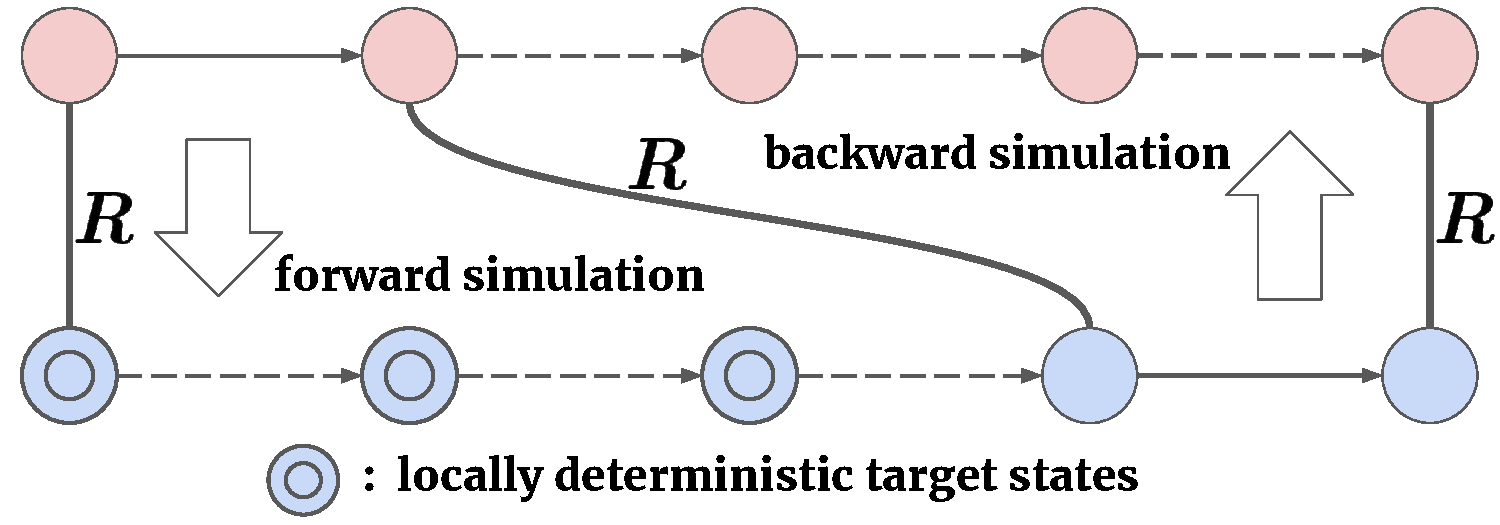
\includegraphics[width=0.7\textwidth]{images/mixed-sim-bold.pdf}
%% 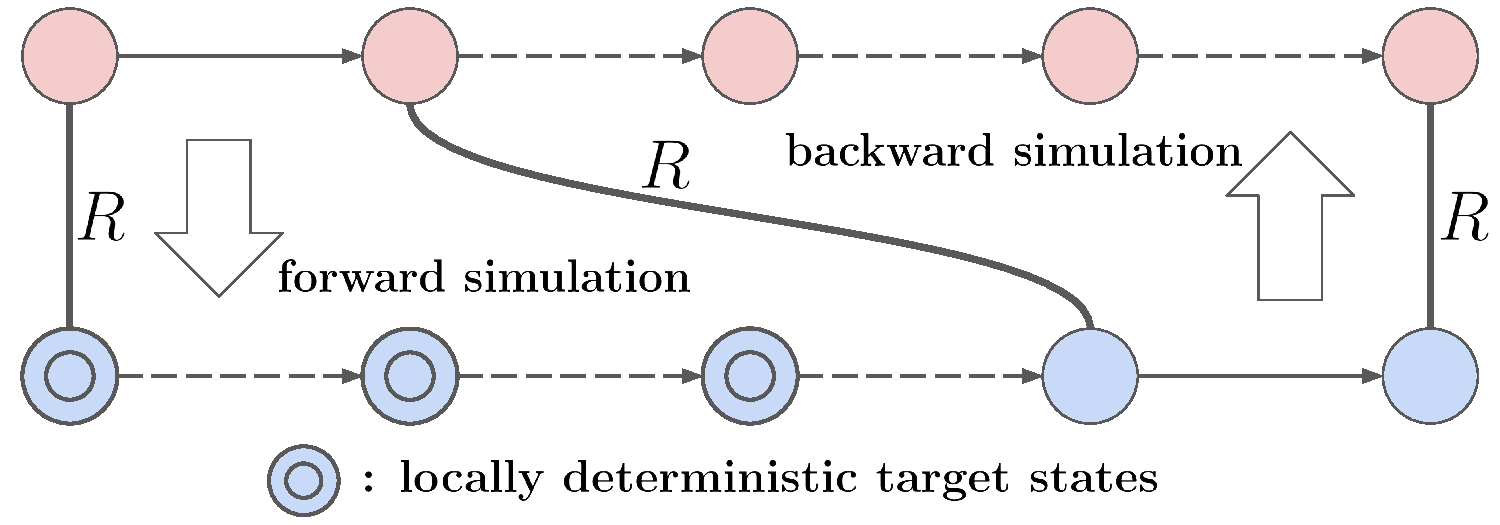
\includegraphics[width=0.7\textwidth]{images/mixed-sim.pdf}
\caption{A visualized example of mixed simulations}
\label{fig:mixedsim}
\end{figure}






\section{Repaired Interaction Semantics}
\label{sec:overview-semantics}

%% We briefly review interaction semantics (\Cref{sec:overview-semantics:background}), discuss the problems (\Cref{sec:overview-semantics:problems}) and present our solutions (\Cref{sec:overview-semantics:solution}).

\subsection{Problems}
\label{sec:overview-semantics:problems}

The problems with the interaction semantics of \ccc{} are that it does
not satisfy two adequacy properties. First, the adequacy w.r.t. C says
that for any C modules $M_1,\ldots,M_n$, the behaviors of the linked
program according to interaction semantics $\beh{M_1 \llink
  \ldots \llink M_n}$ should \emph{be included in} those according to the
physical semantics $\beh{M_1 \plink \ldots\plink M_n}$.  The reason for
failure was quite simple and we could easily fix it: unlike \ccc{}, we allow passing
the \texttt{undef} value to an external module since the C semantics
does so, while we turn ill-typed values into \texttt{undef} when they
are passed to an external module.

Second, the failure of the adequacy w.r.t. assembly is more serious.
Adequacy says that for any assembly modules $M_1,\ldots,M_n$,
the behaviors of the linked program according to interaction
semantics $\beh{M_1 \llink \ldots \llink M_n}$ should \emph{include}
those according to the physical semantics $\beh{M_1 \plink \ldots\plink M_n}$.
Note that the direction is opposite since assembly is the target language.
As discussed before, the reason for failure is that
the interaction semantics of \ccc{} does not have a mechanism to detect
illegal interference and make it undefined behavior~(UB).

\subsection{Our Solution}
\label{sec:overview-semantics:solution}

We identify the sources of inadequacy w.r.t. assembly as violations of
three assumptions made by standard compilers: two on the registers and one on the stack.
We discuss why they 
cause problems with counterexamples and show how to semantically
handle them without changing the underlying language semantics.

\subsubsection{Assumptions on the Registers}
\label{sec:overview-semantics-register}
%
The two problematic assumptions on the registers are that
an invoked assembly function $(i)$ should
preserve the initial values of the callee-save registers, and $(ii)$
should not access the memory via the leftover pointer values remaining
in those registers that are not involved in passing meaningful information to the callee,
which we henceforth call \emph{\nip{}} registers.

\begin{figure}[t]
\fbox{\begin{minipage}{.8pc}\mbox{}\\[13.53mm](a)\\[11.73mm]\mbox{}\end{minipage}}
\hspace*{-1.9mm}
\begin{minipage}{0.55\textwidth}
\begin{Verbatim}[frame=single]
int main()   {          main:
  int* x = malloc(8);     ...
  x[0] = 0;               *(%rbx) = 0;
  x[1] = 1;               *(%rbx + 4) = 1;
  f();               -->  f();
  out(x[0]);              out(*(%rbx));
  ...                     ...
}
\end{Verbatim}
\end{minipage}
$\mbox{}~\mathlarger{\mathlarger{\mathlarger{\mathlarger{\mathlarger{\llink}}}}}~\mbox{}$
\fbox{\begin{minipage}{.8pc}\mbox{}\\[9.33mm](b)\\[7.53mm]\mbox{}\end{minipage}}
\hspace*{-1.9mm}
\begin{minipage}{0.28\textwidth}
\begin{Verbatim}[frame=single]
f:
  if (g(%rbx))
    %rbx = %rbx + 4;
  else
    *(%rbx) = 1;

\end{Verbatim}
\end{minipage}
\caption{A counterexample showing the problem with the assumptions on the registers}
\label{fig:reg-convention}
\end{figure}

\myparagraph{Counterexamples}
%
The example in \Cref{fig:reg-convention} shows how violations of the two
assumptions can invalidate correct compiler translations.
%
The code in the left box~(a) shows a standard translation of C code into assembly
(written in pseudocode) performed by mainstream compilers like GCC and LLVM, where the accesses to
the array \texttt{x} are translated into accesses via the register
\texttt{\%rbx} assuming that \texttt{\%rbx} is set to contain the
address of \texttt{x}. An important point here is that the compiler
assumes that $(i)$ the value of \texttt{\%rbx} is unchanged across
the function call \texttt{f()} since it is a callee-save register,
and also $(ii)$ the values in the array pointed to by \texttt{\%rbx} are
unchanged across \texttt{f()} since the array's addresses do not escape
except via \nip{} registers like \texttt{\%rbx}.
Therefore, the compiler expects that \texttt{out(*(\%rbx))} in the target code
correctly outputs \texttt{0}.

The right box~(b) presents an example of handwritten assembly
(written in pseudocode) for function \texttt{f} that violates the
above two assumptions of the compiler. The code either increments
\texttt{\%rbx} by \texttt{4} or writes \texttt{1} to \texttt{*(\%rbx)}
depending on the result of call to \texttt{g}.  Now if we link the assembly
code in (a) and that in (b) together, one can easily see that
\texttt{out(*(\%rbx))} incorrectly outputs~\texttt{1} instead
of \texttt{0} in either case: in the former case, \texttt{\%rbx}
points to the second element of the array~\texttt{x}, which contains
\texttt{1}; in the latter case, the value of \texttt{*(\%rbx)} is
directly updated to \texttt{1}. Therefore, it makes sense to
define those illegal behaviors of (b) as undefined behavior~(UB).

\myparagraph{Our Model}
%
We present our model making the illegal behaviors UBs
in stages, explaining at each stage why naive models do not work.

First, in order to enforce the preservation of callee-save register
values, we store the initial values of the callee-save registers at
the \texttt{init-core} step of assembly modules; and check, at the
\texttt{halted} step, whether the final values of those registers are
equal to the stored initial values and if not, raise UB.  Here, the
question is, when a new core with a fresh register file is pushed into the core stack,
what values should be set as initial values of the \nip{}
registers including all of the callee-save registers.  Since the
registers may contain arbitrary values in the physical assembly
semantics, a natural choice would be to initially set them to contain
the \texttt{undef} value, which is an abstract value representing all
possible values. Indeed, this is the choice of \ccc{}.  However, there
is a serious problem. Since, for instance, \texttt{undef + 4} results
in \texttt{undef}, checking whether the final values of callee-save
registers are equal to the initial values, \ie \texttt{undef}, is
not sufficient. Specifically, the assembly code in (b) above
does not raise UB in this new semantics in case \texttt{g(\%rbx)} returns \texttt{1}
because the initial and final values of \texttt{\%rbx}
are both \texttt{undef} and thus equal
even though the callee-save register \texttt{\%rbx} is incremented
by \texttt{4} in the physical semantics.

Second, another natural solution would be to initially set the
\nip{} registers to nondeterministically contain arbitrary
values including \texttt{undef}. Though this model is more flexible,
it still has a problem. For instance, in the above example, to
simulate the physical behaviors of the assembly function \texttt{f} in
interaction semantics, one can set the initial value of \texttt{\%rbx} to
be either $(i)$ \texttt{undef} (\ie a more abstract value than the physical one), or
$(ii)$ a pointer to the array \texttt{x} (\ie a value equivalent to the physical one):
other values cannot be used since they are not refined by the value of \texttt{\%rbx} in the target,
which is required since the value is passed to an unknown function~\texttt{g}.
In the former case, if
\texttt{g(\%rbx)} returns \texttt{1}, we have the same problem with
callee-save checking as shown above.  In the latter case, if
\texttt{g(\%rbx)} returns \texttt{0}, the function \texttt{f}
successfully updates the array~\texttt{x} thereby invaliding the
translation in (a) as illustrated above.

We solve this problem by further revising the second model:
nondeterministically allocating an arbitrary number of \emph{junk
  blocks} (\ie blocks of size zero) and then initializing the
\nip{} registers with arbitrary non-pointer values or
\emph{junk pointers} (\ie pointers to the junk blocks).  Then we can
simulate the physical behaviors by initializing each register $r$
$(i)$ with the same non-pointer value if the physical value of $r$ is
a non-pointer value; and $(ii)$ otherwise with a fresh junk pointer.
The high-level idea is that, like \texttt{undef}, a junk pointer is
more abstract (\ie causing more UBs) than any pointer but, unlike
\texttt{undef}, sufficiently distinguishable. For instance,
in the previous example, if \texttt{g(\%rbx)} returns \texttt{1},
the initial and final values of \texttt{\%rbx} (\ie $p$ and $p+4$ for a junk pointer $p$)
are distinguished thereby raising UB by the callee-save checking;
if \texttt{g(\%rbx)} returns \texttt{0},
the memory access \texttt{*(\%rbx) = 1} raises UB because \texttt{\%rbx}
points to a junk block of size zero.

Finally, note that introducing nondeterminism as above is not a
showstopper thanks to the mixed simulation, as discussed in
\Cref{sec:overview-verification:mixedsim}: we can do forward
simulation everywhere except for the \texttt{init\_core} step of
assembly modules, where we should do backward simulation.

\subsubsection{Assumptions on the Stack}
\label{sec:overview-semantics-memory}
%
The problematic assumption on the stack is that the
\emph{outgoing arguments area} of a caller's stack (\ie where overflowing function
arguments are stored) should be fully \emph{owned} by the callee. In
other words, the callee can assume that the arguments area is never
modified by others unless its addresses are revealed to the public by
the callee itself.

\begin{figure}[t]
\fbox{\begin{minipage}{.8pc}\mbox{}\\[9.33mm](a)\\[7.53mm]\mbox{}\end{minipage}}
\hspace*{-1.9mm}
\begin{minipage}{0.255\textwidth}
  \begin{Verbatim}[frame=single]
main:
  ...  
  leak = %rsp;
  f(..., 0);
g:
  *leak = 1;
  \end{Verbatim}
\end{minipage}
$\mbox{}~\mathlarger{\mathlarger{\mathlarger{\mathlarger{\mathlarger{\llink}}}}}~\mbox{}$
\fbox{\begin{minipage}{.8pc}\mbox{}\\[9.33mm](b)\\[7.53mm]\mbox{}\end{minipage}}
\hspace*{-1.9mm}
\begin{minipage}{0.595\textwidth}
  \begin{Verbatim}[frame=single]
void f(..., int64_t x)       f:
{                              ...
  out(x);                      out(*(%rax));
  g();                  -->    g();
  out(x);                      out(*(%rax));
}                              ...
  \end{Verbatim}
\end{minipage}
\\[1mm]
\fbox{\begin{minipage}{.8pc}\mbox{}\\[17.53mm](c)\\[16.73mm]\mbox{}\end{minipage}}
\hspace*{-1.9mm}
\begin{minipage}{.95\textwidth}
\fbox{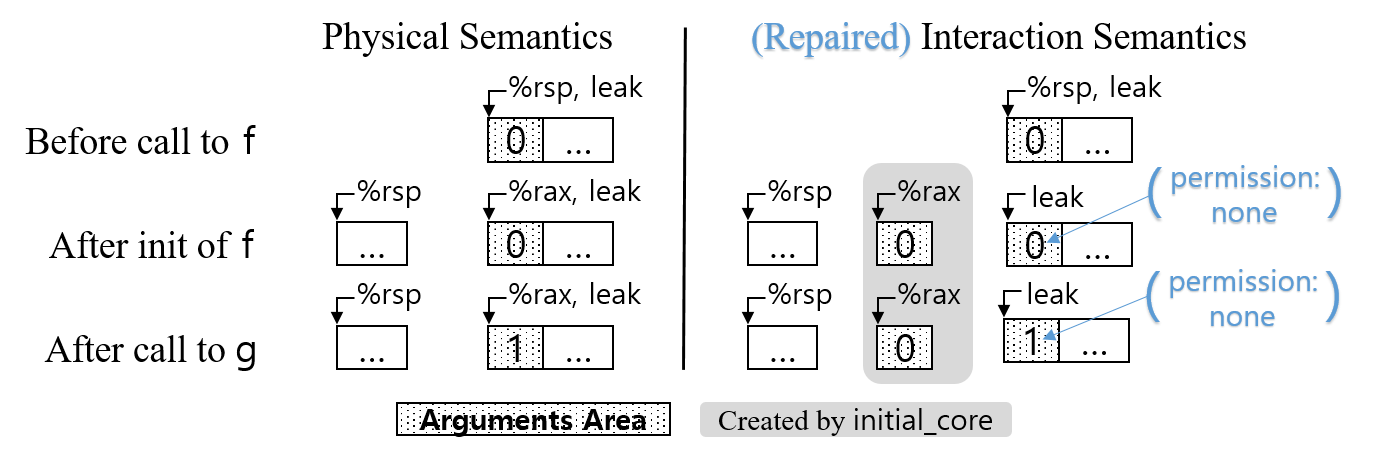
\includegraphics[width=.983\textwidth]{images/ex-stack.png}}
\end{minipage}
\caption{A counterexample showing the problem with the assumption on the stack}
\label{fig:stack-convention}
\end{figure}

\myparagraph{Counterexamples}
%
The example in \Cref{fig:stack-convention} shows how violations of the assumption
can invalidate correct compiler translations.
%
The box~(a) shows handwritten assembly code implementing two functions
\texttt{main} and \texttt{g}; the box~(b) shows a standard translation
of C code into assembly essentially performed by \texttt{gcc -O0}; and
the left-hand side (LHS) of the box~(c) depicts the shape of the stack
during execution in the physical semantics.
The function \texttt{main} stores the address of the
outgoing arguments area (\ie \texttt{\%rsp} as depicted in LHS of (c))
in the global variable \texttt{leak} and invokes the function
\texttt{f}, where the last argument \texttt{0} is stored in the
arguments area of the stack. Then the function \texttt{f} makes three
function calls, \texttt{out(x)}, \texttt{g()} and \texttt{out(x)},
where the argument \texttt{x} is directly read from the arguments area
pointed to by \texttt{\%rax} in the assembly, as depicted in LHS of
(c), and \texttt{out(x)} outputs the read value.  Finally, the
function \texttt{g} updates the arguments area pointed to by
\texttt{leak} with~\texttt{1}, as depicted in LHS of (c), between the
two function calls \texttt{out(x)}.

An important point here is that the compiler assumes that the
arguments area (\ie \texttt{\%rax}) is unchanged across the
function call \texttt{g()} since it is fully owned by \texttt{f}.
Therefore, the compiler expects that both calls
\texttt{out(*(\%rax))} in the target code correctly output
\texttt{0}. However, since the function \texttt{g} updates the
arguments area with \texttt{1} via \texttt{leak}, the two calls
incorrectly output \texttt{0} and~\texttt{1}.
We confirmed this incorrectness by
compiling \texttt{f} with \texttt{gcc -O2}, which
eliminates the second load \texttt{*(\%rax)} by propagating
the result of the first load across \texttt{g()}
thereby outputting \texttt{0} twice.

\myparagraph{Our Model}
%
In order to solve the problem, we have to distinguish accesses to the
arguments area via the caller from those via the callee and define the
former as UB. Though making such distinction is difficult in the
physical semantics, fortunately it is already made in interaction
semantics due to the language-independent design. For example, consider
the interaction semantics of the above example, depicted in the
right-hand-side (RHS) of \Cref{fig:stack-convention}~(c).  The
difference is that when the assembly function \texttt{f} is invoked,
the initialization process (\ie \texttt{init\_core}) of the module
semantics newly constructs the arguments area of the stack from the
given logical arguments in order to make an environment needed to
execute the assembly function \texttt{f}. This is essentially needed
because the caller may not be an assembly module so that it may not
have its own stack at all.  Then the callee sees the new arguments
area created by \texttt{init\_core} while the caller (in assembly)
sees the original arguments area.

Although the original interaction semantics does not prevent access to
the arguments area via the caller, we can easily fix it.
We simply $(i)$ turn off the access
permission of the original arguments area in the \texttt{at\_external}
step of the caller module, and $(ii)$ turn it back on in the
\texttt{after\_external} step. Note that the notion of permission
%% is already an existing feature of
already exists in the \cc{} semantics, so that we do not
need to strengthen it. In the above example again,
the update by \texttt{g} will raise UB since the original argument area pointed
to by \texttt{leak} has no access permission.





%%% Local Variables:
%%% mode: latex
%%% TeX-master: "main"
%%% End:
